\documentclass{article}
\usepackage[utf8]{inputenc}
\usepackage{graphicx}
\setlength{\parindent}{0pt}
\setlength{\parskip}{1em}

\title{FOAR705 - Proof of Concept Elaboration II}
\author{Jan Jugueta - 44828020}
\date{5th of September 2019}

\begin{document}

\maketitle

\section*{Research Topic}

Alot has changed in the past week in relation to my Masters of Research thesis. During that time, I have had several meetings with different academic lecturers and mentors. I believe this is the first time that I had a clear idea of what Masters of Research topic will be, along with what specific sources I will use.

My research will focus on how the East German state used their state-owned media in the lead up to the 1974 FIFA World Cup. This particular World Cup is of significance to both West and East Germany, because the World Cup finals were to be held in West Germany, whilst it would the first time that East Germany would compete in the finals. To top it all off, East Germany were drawn to play West Germany in the group stage.

This research will involve obtaining newspaper articles about the World Cup from \textit{Neues Deutschland}, the pre-eminent East German newspaper. The search will limit itself to the year leading up to the World Cup till the end of 1974. A semiotic analysis of the articles content will also be performed. With these two distinct steps, I then propose two different Proof of Concepts. 

I have not entirely decided to throw away my old Proof of Concept proposed in Scoping II, however, I do feel that this proposal will be more beneficial to my workflow.

\section*{Computational Analysis}

As I have changed my research question, my research method has invariably changed. I now know exactly what sources I will be working with.

\subsection*{Decomposition}

There are two main tasks for this project. The first is collecting the newspaper articles and the second is to analyse the articles. The process can be decomposed into these smaller items:

\begin{itemize}
    \item identifying a date search range
    \item identifying key search terms
    \item sorting out irrelevant news articles
    \item downloading the text from the newspaper articles onto my machine
    \item storing the articles in a directory on my machine
    \item labelling and tagging articles for ease of re-use
    \item uploading the articles to a text analysis website
    \item interpreting the textual analysis
    \item identify key themes from the analysis
\end{itemize}

\subsection*{Pattern Recognition}

Identifiable patterns include:

\begin{itemize}
    \item the repetition of the search process when using a new search term (including the sorting out of irrelevant articles, downloading articles and storing them in a directory)
    \item the repetition of the process to uploading the articles to a world analysis website
    \item the repetition of the process to log and key findings that may emerge from the textual analysis
\end{itemize}

\subsection*{Algorithm}

The likely method for this research is as follows:

\begin{enumerate}
    \item Access web archive of the newspaper
    \item Delimit search time period (i.e. 1/1/1973 - 31/12/1974)
    \item Enter search term in the search window
    \item Sort out relevant and irrelevant newspaper articles
    \item Download (or copy) the text from the newspaper article
    \item Save the text onto a .txt file on my machine
    \item Tag metadata information of the article including publish date, authors name and location
    \item Organise articles by date (or theme, I have not yet decided which is best)
    \item Upload the corpus of text to textual analysis website
    \item Identify themes that emerge from the analysis
    \item Note down findings in research journal.
\end{enumerate}


\section*{Elaboration}

Building on the work done in Scoping I\&II and Elaboration I, I have found some technologies that can help with the research process. When reviewing Elaboration I, I discovered there were actually three main tasks involved in my research process proposal.

\begin{enumerate}
    \item Finding of sources and downloading the articles from \textit{Neues Deutschland} (including the storing of sources on my machine)
    \item Textual Analysis
    \item Note organisation
\end{enumerate}

\newpage
\section*{Finding and downloading newspaper articles from \textit{Neues Deutschland}}

\begin{figure}[h]
    \centering
    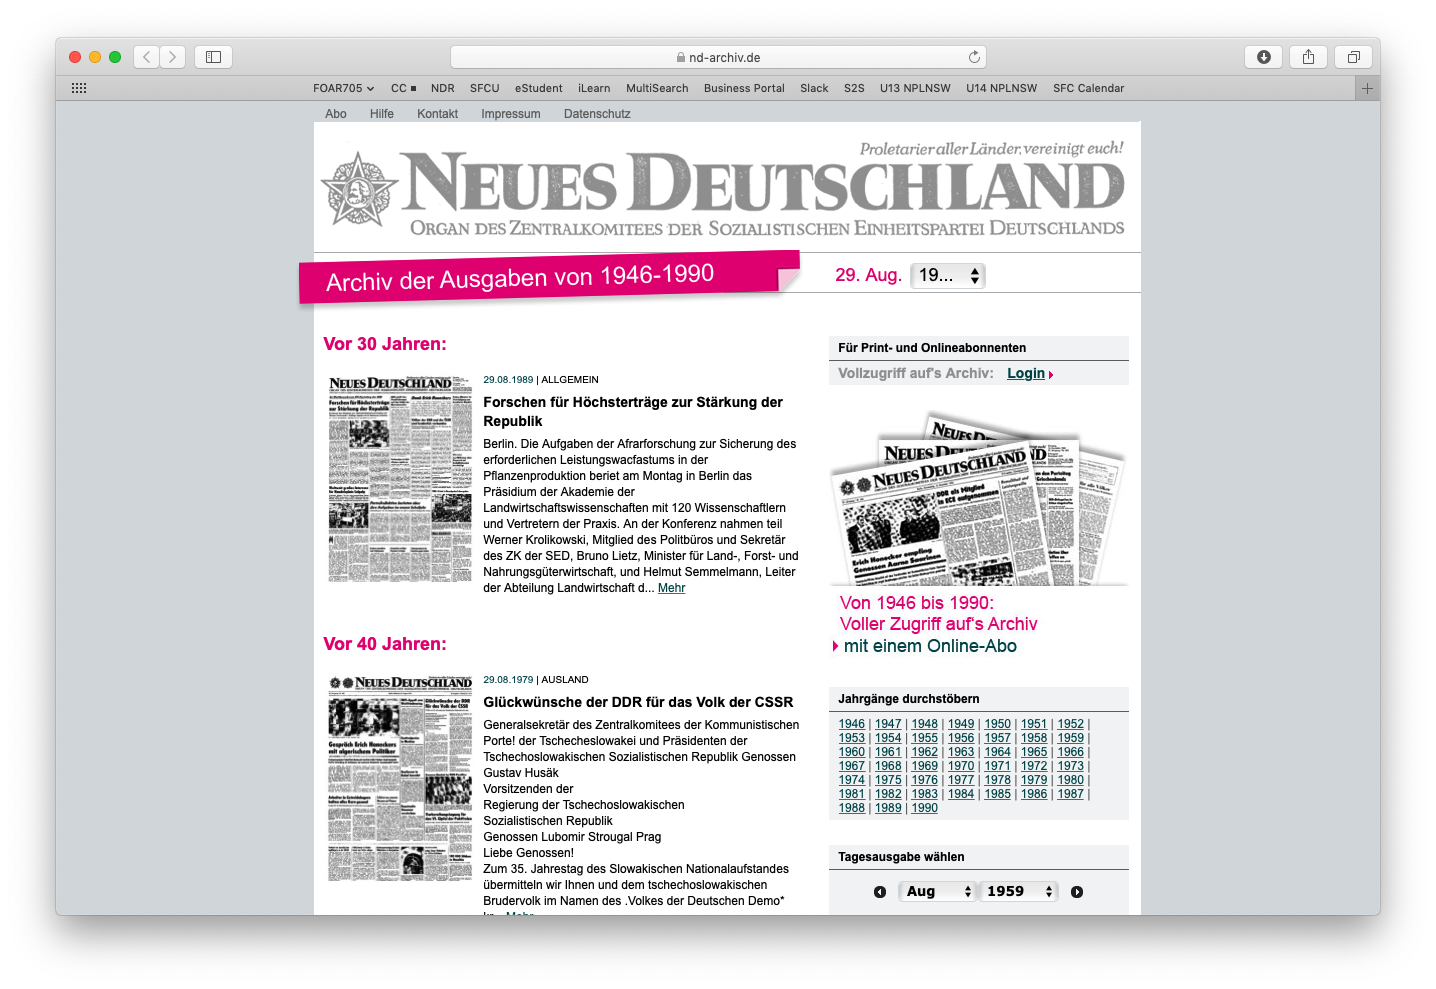
\includegraphics[width=\textwidth]{nd.png}
    \caption{\textit{Neues Deutschland website}}
    \label{fig:my_label}
\end{figure}


\textit{Neues Deutschland} was an organ for the Central Committee of the Socialist United Party in East Germany. The website nd-archiv.de contains all newspaper articles published by the magazine from 1946 to 1990.

Having learnt of APIs in last weeks class, I looked if there any available for \textit{Neues Deutschland}, but alas there were none available. This will mean this process of data collection will be performed 'manually'. 

\textbf{Objective:} Find all articles with the term \textit{Weltmeisterschaft} (World Cup) between January 1st 1973 and December 31st 1974 and save the text on my machine.

\begin{enumerate}
    \item Enter 'weltmeisterschaft' in the \textit{Suchausdruck}.
    \item Change the date range from 1st January 1973 to 31st of December 1974 in the \textit{In welchem Zeitraum} field.
    \item Leave all other fields to default setting.
    \item Click \textit{Suchen}.
\end{enumerate}

\begin{figure}
    \centering
    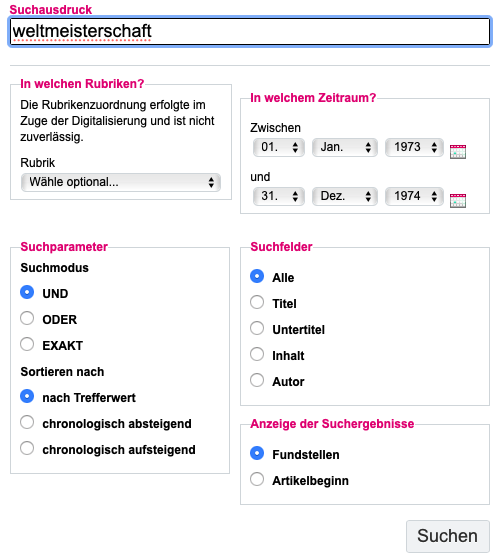
\includegraphics[width=\textwidth]{nd_search.png}
    \caption{\textit{Search Window}}
    \label{fig:my_label}
\end{figure}

From this search result, we can see that it has returned more than 100 articles that match the criteria we have entered.

\begin{figure}
    \centering
    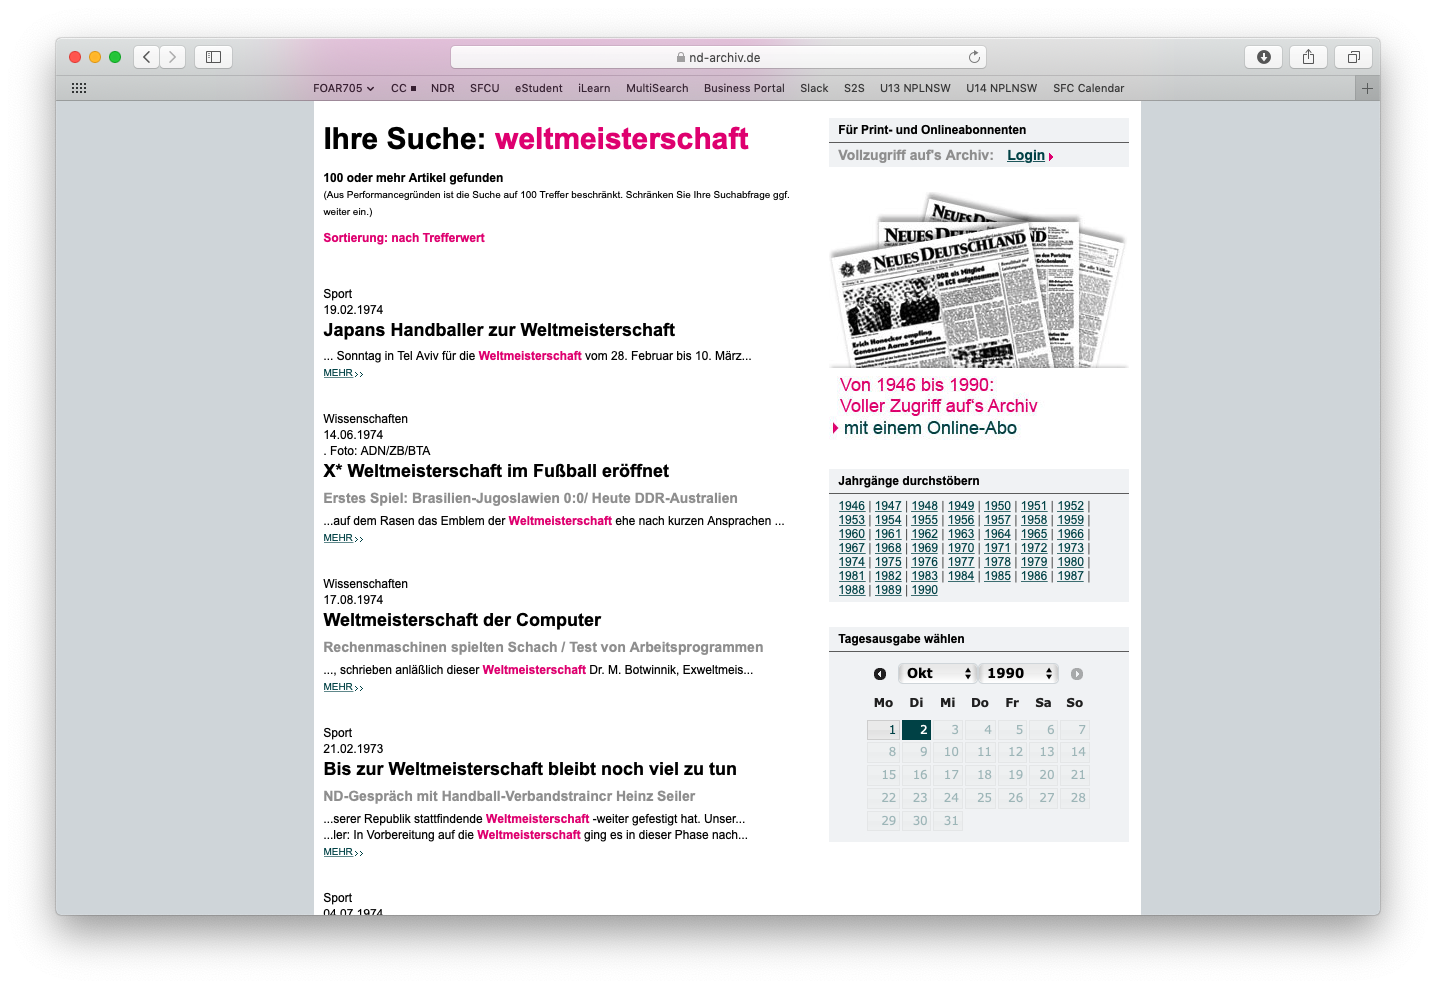
\includegraphics[width=\textwidth]{nd_searchresult.png}
    \caption{Search Result}
    \label{fig:my_label}
\end{figure}

Here comes the part of the process that becomes rather repetitive. The process is as follows.

\begin{enumerate}
    \item Click on the first article returned in the result.
    \item Copy the text from the article into a .txt (or .rtf) file.
    \item Save and name the .txt (or .rtf) into a directory stored on my machine.
    \item Go back to the website and continue this process with the next search result.
    \item Continue this process until all articles are copied.
\end{enumerate}

Once this process is completed, I should have all articles that reference 'Weltmeisterschaft' on my computer.

\textbf{Result:} Articles found relating to the search term 'Weltmeisterschaft'. Text saved onto .txt files in a directory on my machine.

\newpage
\section*{Textual analysis of the corpus using Voyant Tools}

\textbf{Objective:} Use Voyant Tools to perform textual analysis on the corpus of text.

For testing this concept, I have created .rtf files in a directory on my machine that contain German-text articles about football.

\begin{figure}[h!]
    \centering
    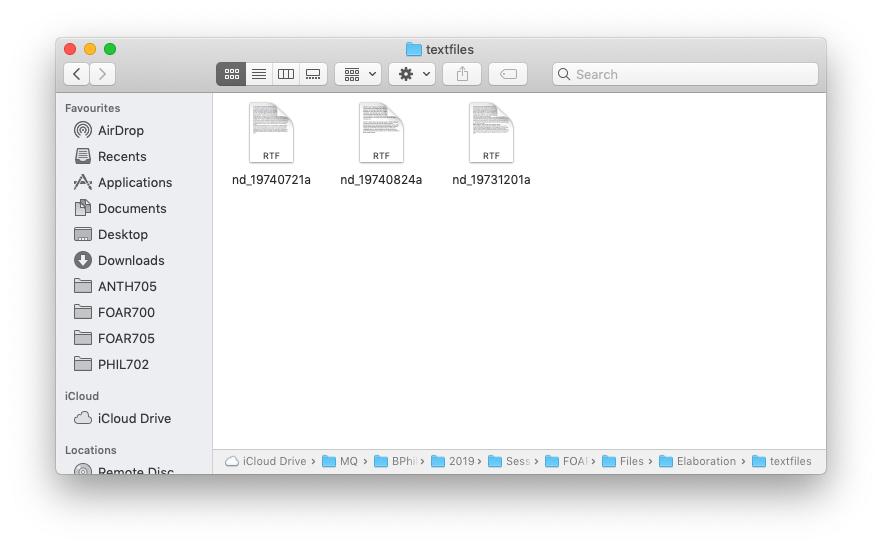
\includegraphics[width=\textwidth]{textfiles.png}
    \caption{Directory with .rtf files on my computer}
    \label{fig:my_label}
\end{figure}

Using the 'upload' function on the Voyant Tools website, I can select all my corpus files and have them analyzed by Voyant Tools.

\begin{figure}[h!]
    \centering
    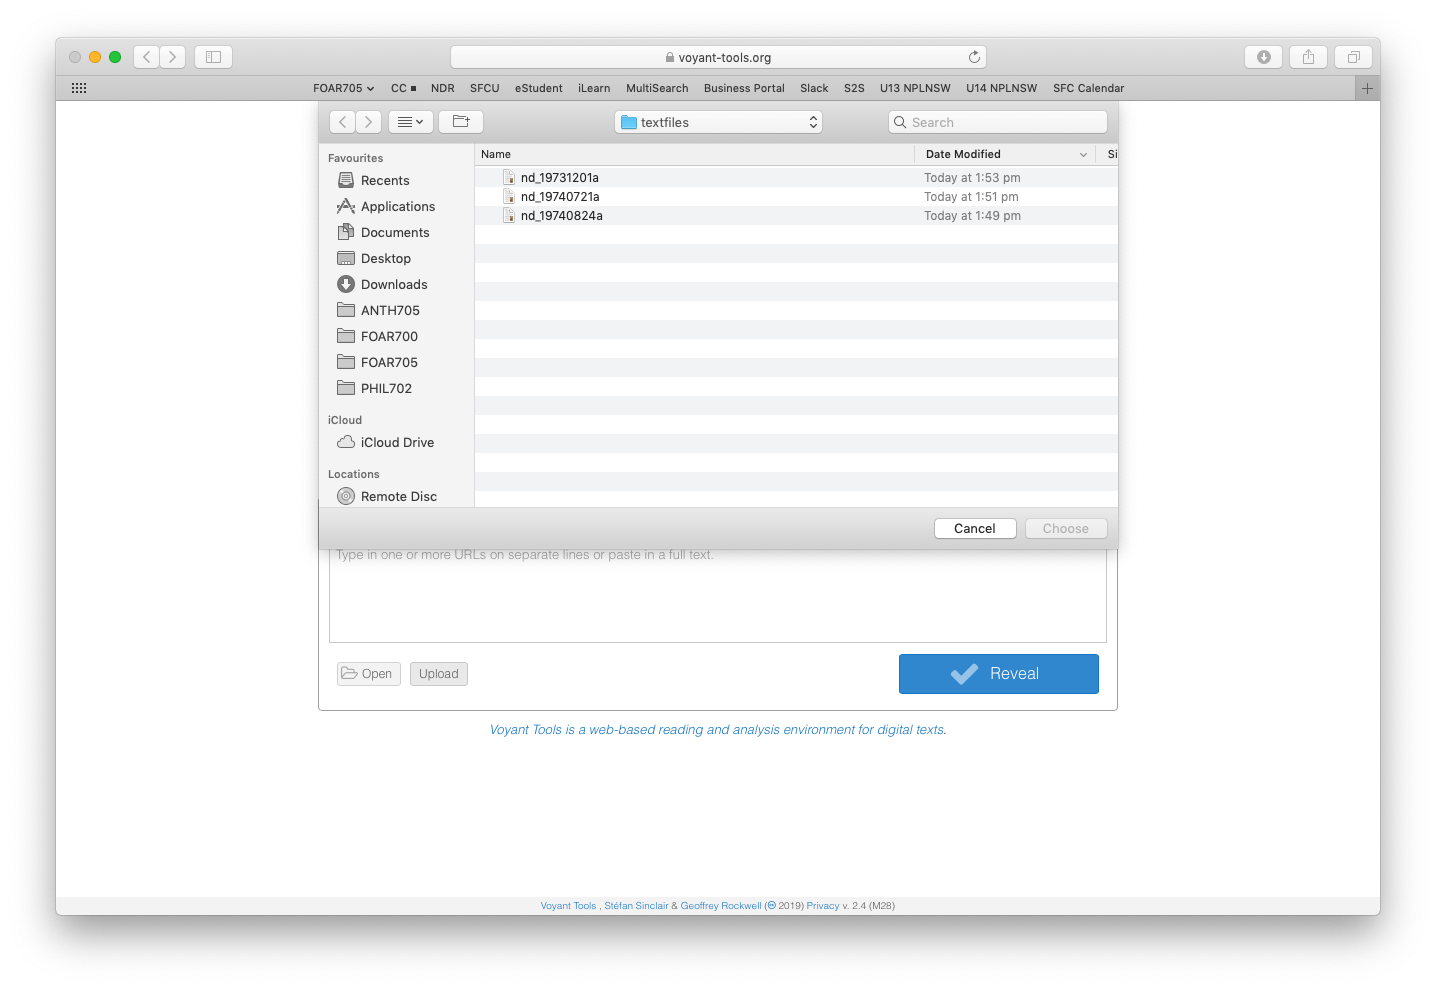
\includegraphics[scale=0.15]{voyantupload.png}
    \caption{Voyant Tools upload window}
    \label{fig:my_label}
\end{figure}

Once uploaded, I can use Voyant to analyze the corpus a number of ways. I have yet to decide which specific methodology I will employ, however, it is more than likely that Voyant will be beneficial whichever way I choose to go.

\begin{figure}[h!]
    \centering
    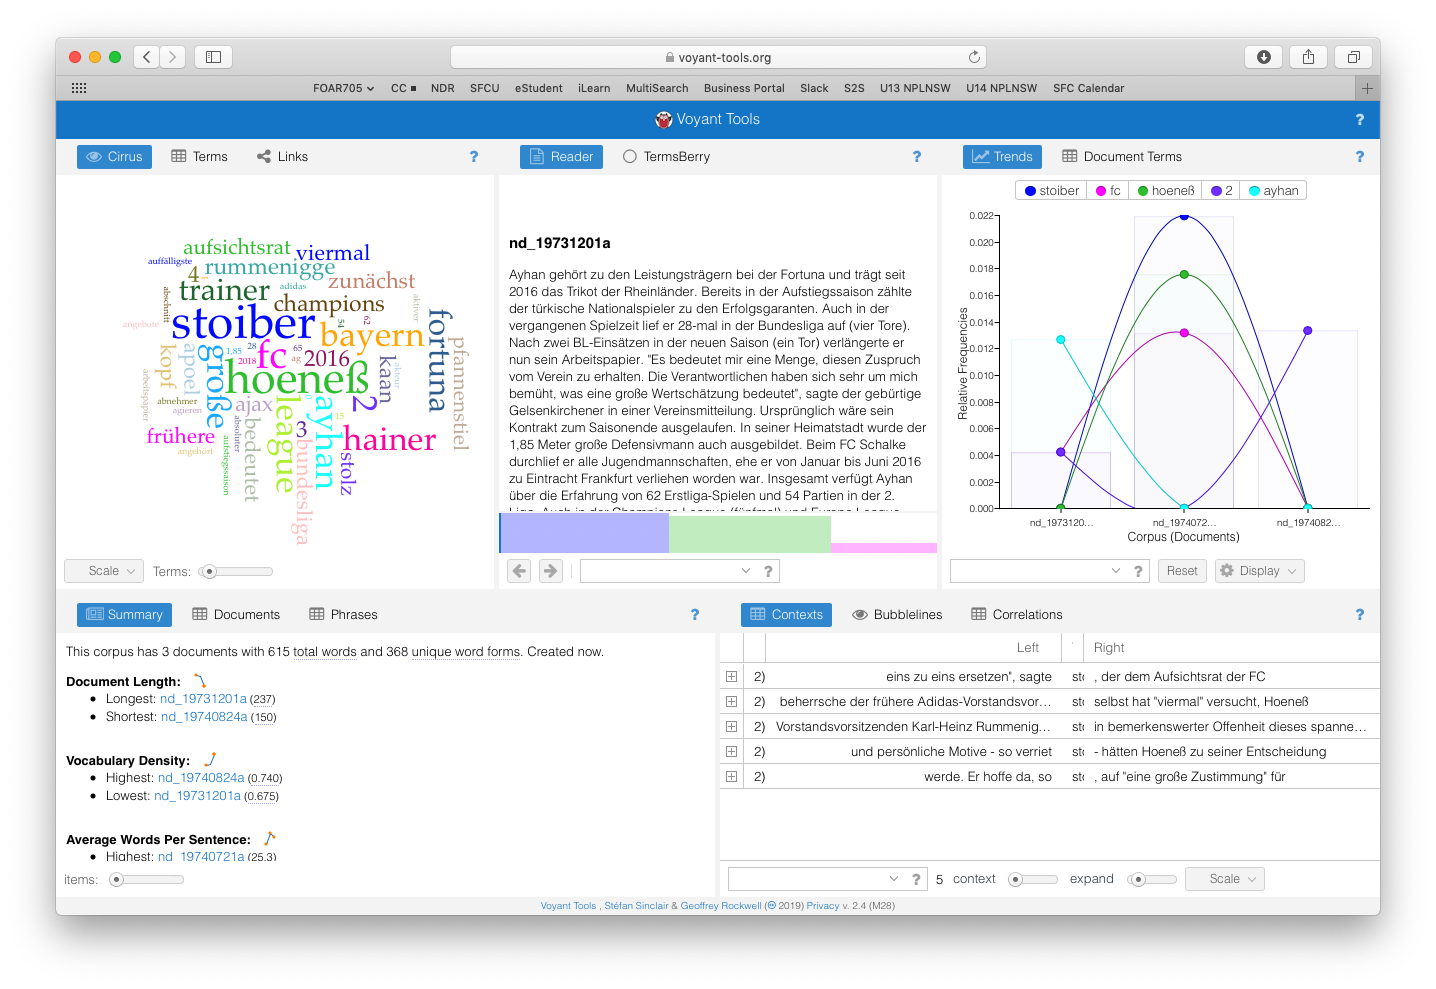
\includegraphics[width=\textwidth]{voyantresult.png}
    \caption{Voyant Tool's analysis of the corpus.}
    \label{fig:my_label}
\end{figure}

\textbf{Result:} Voyant Tools was able to analyse the corpus of text (collection of articles). This will be useful in analysing text over a long period of time.

\newpage
\section*{Note Organisation}

I have considered two possible solutions for taking notes. Microsoft's OneNote or simply saving my notes in separate .txt files in a directory.

\textbf{Objective:} Store notes on machine in a way that is organised and easy to recall.

\subsection*{Microsoft OneNote}

I have been using OneNote ever since the first year of my undergraduate degree at Macquarie University. I initially chose to use OneNote because I work across several machines and devices and liked how easily it synced up. I have also organised many of my units in such a way that the notes are easily categorised. For this MRes project, I would do something similar. Of particular use to me will be the tagging option. This would allow me to recall notes on things quickly.

\begin{figure}[h!]
    \centering
    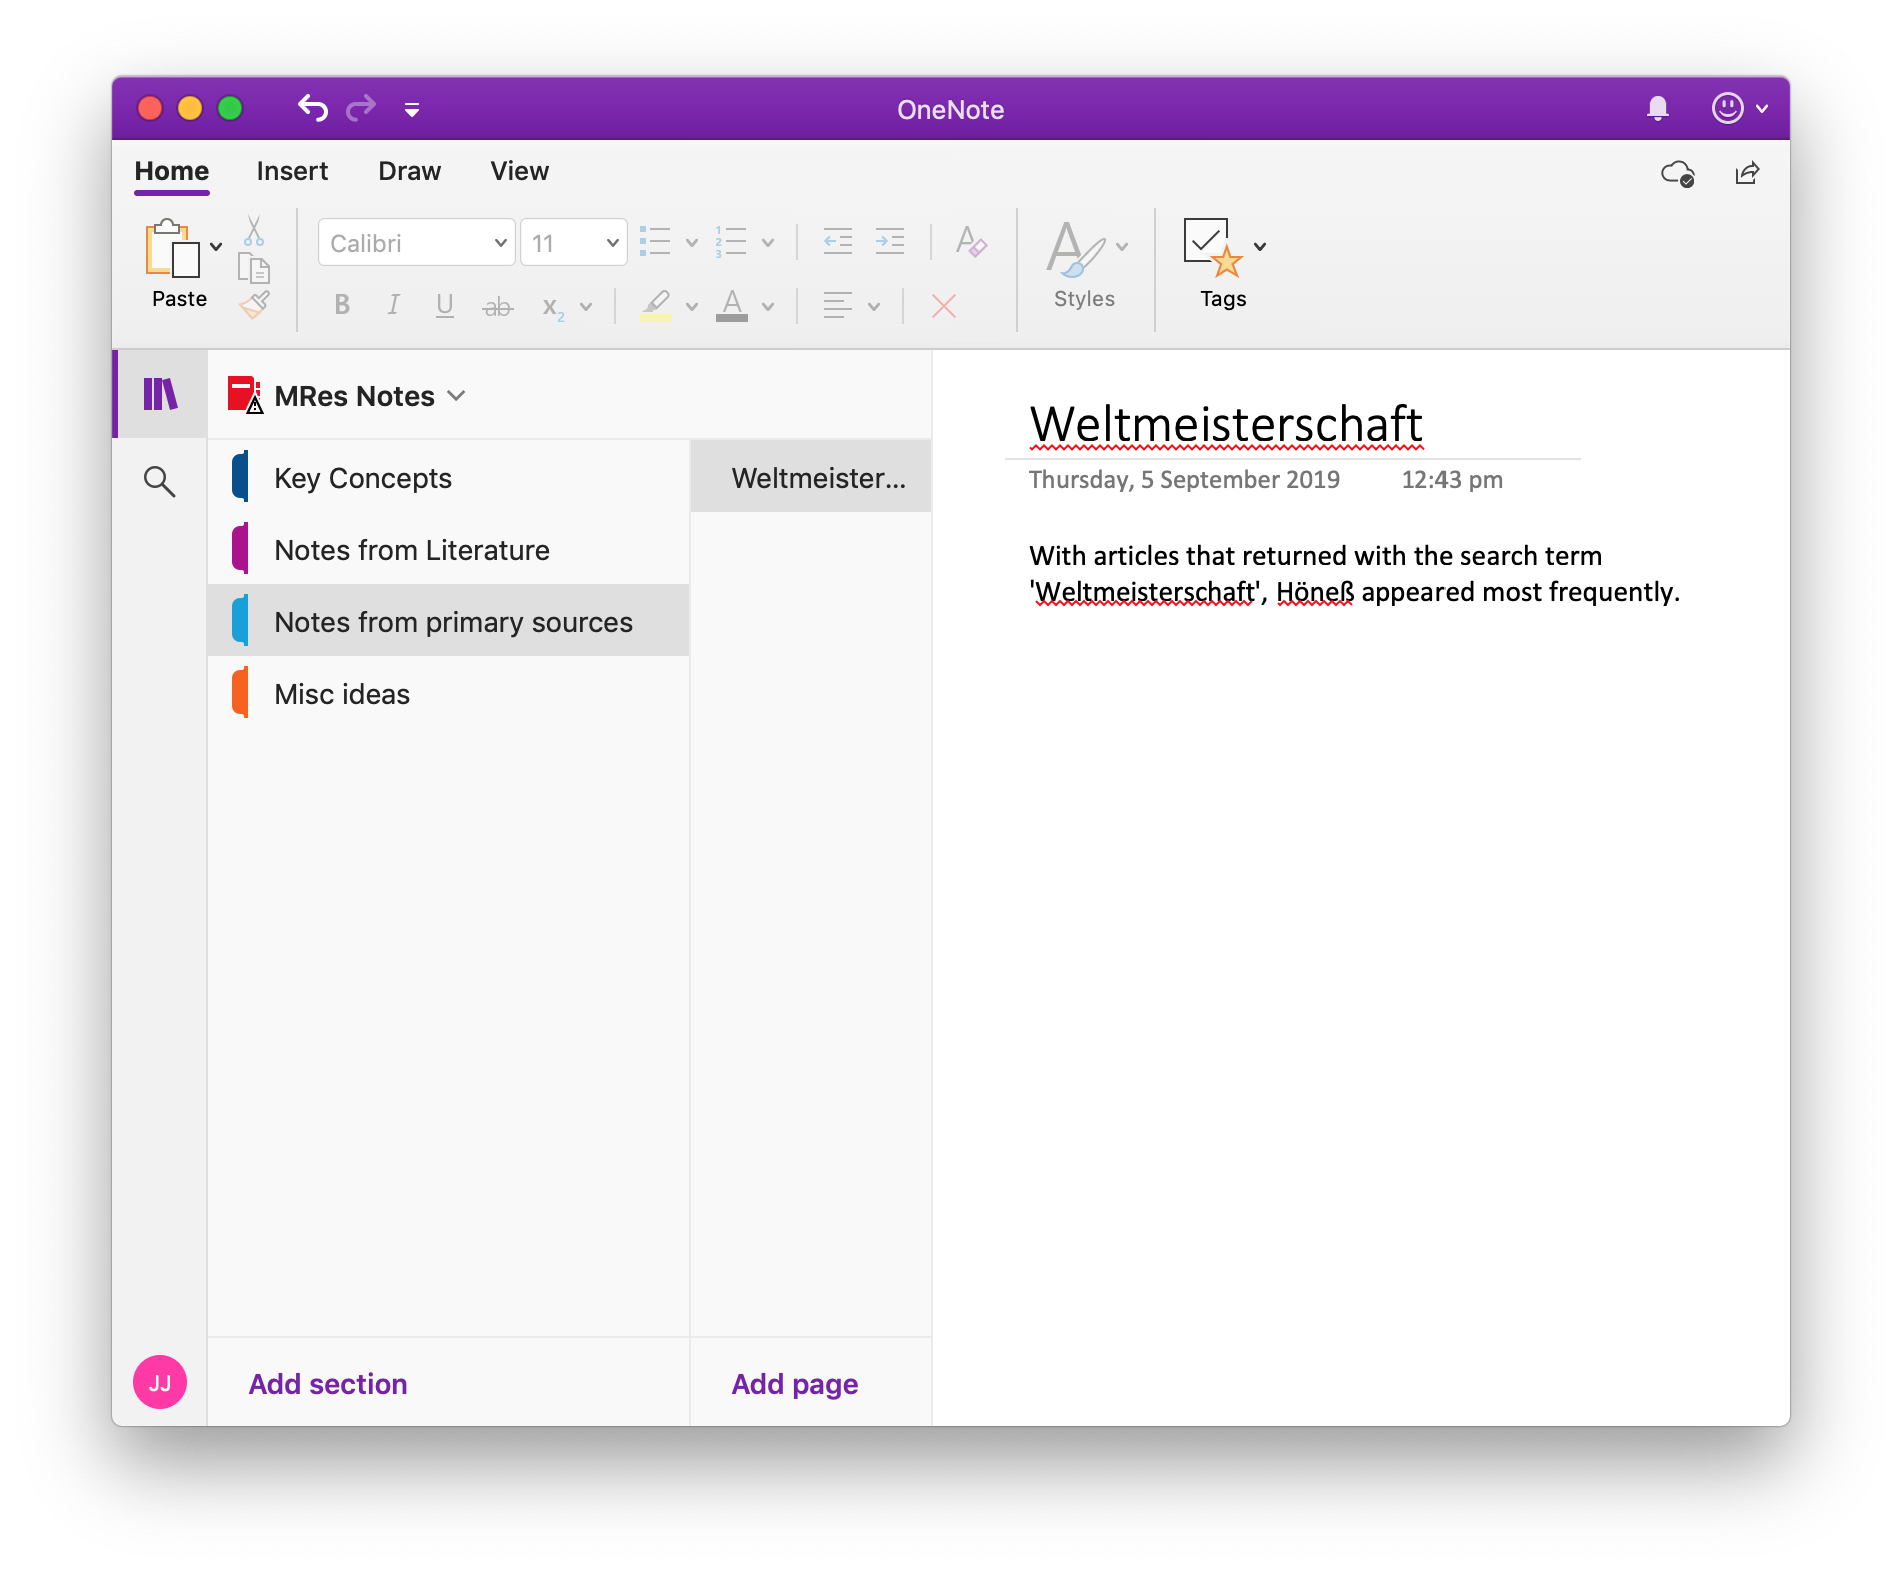
\includegraphics[width=\textwidth]{onenote.png}
    \caption{Proposed organisation in OneNote for MRes project.}
    \label{fig:my_label}
\end{figure}

\subsection*{Storing notes as text files}

Using a text file, notes could be stored in a similar fashion as it is done with OneNote. However, syncing is not an option (unless using a cloud based service) and there is no tagging. 

\begin{figure}[h!]
    \centering
    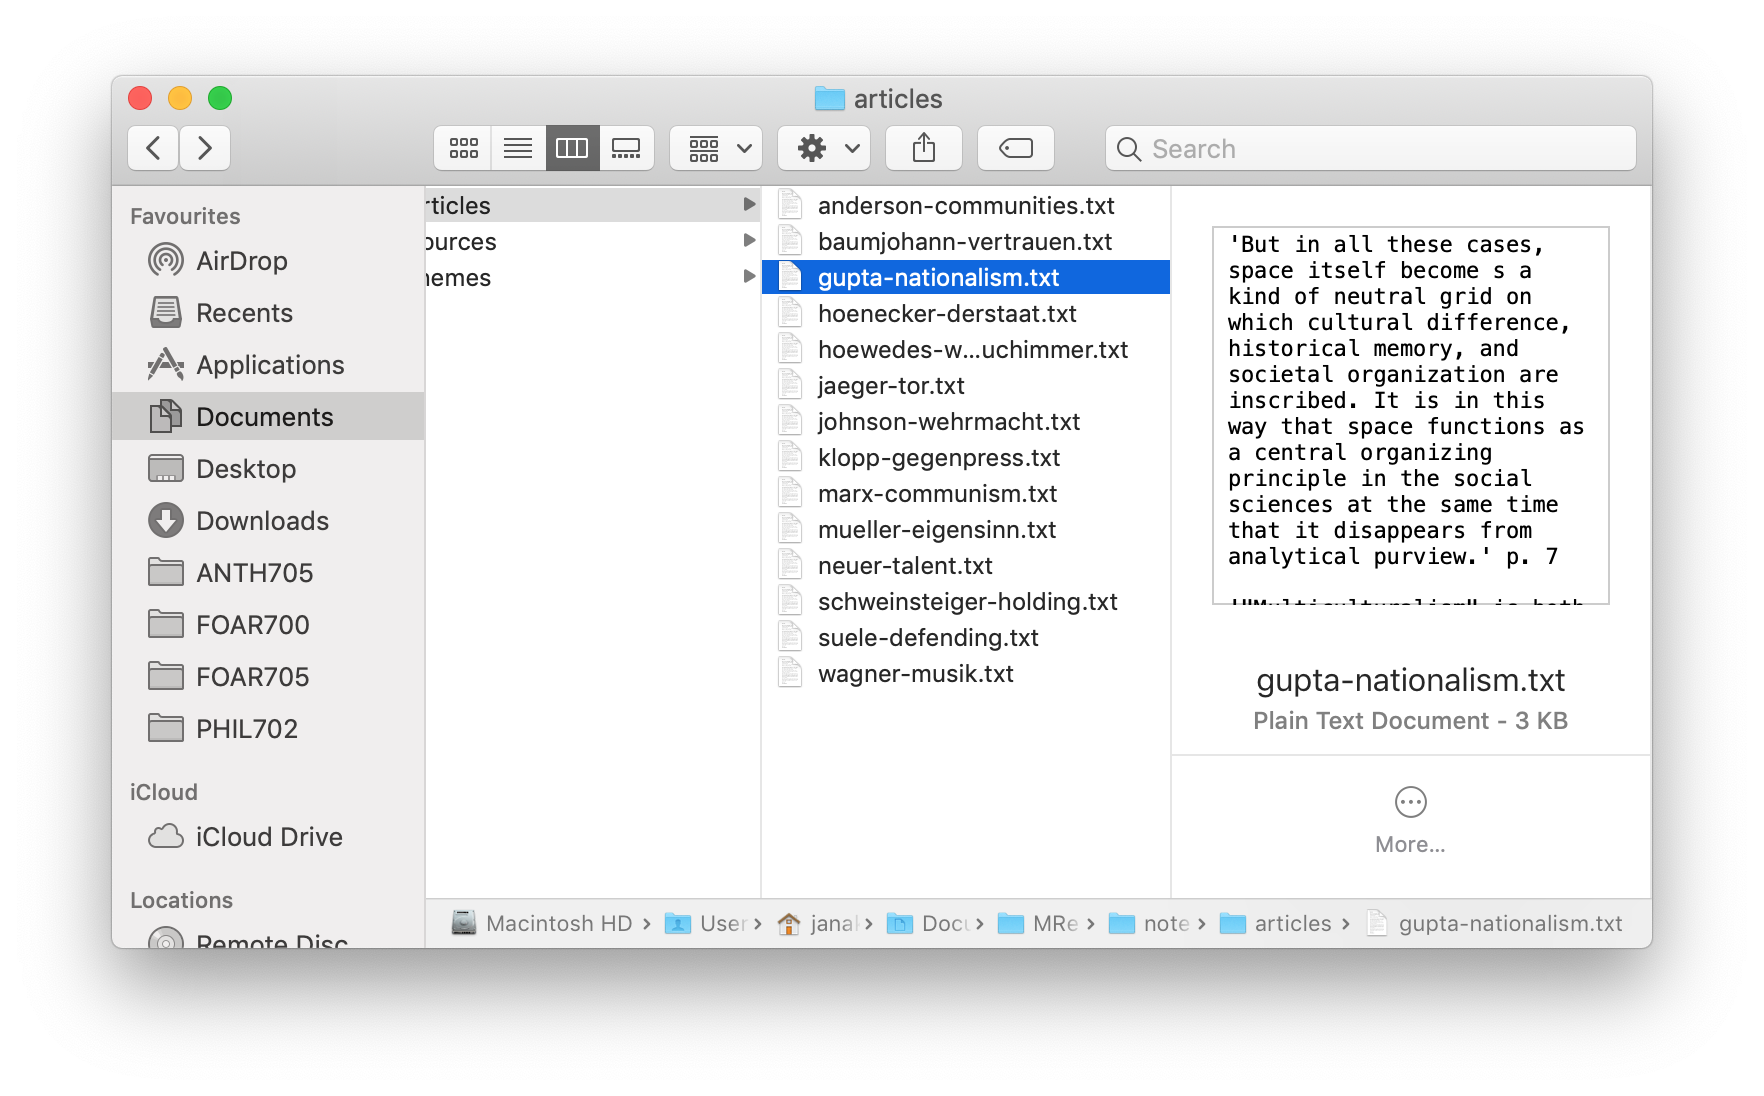
\includegraphics[width=\textwidth]{text.png}
    \caption{Proposed organisation directories with .txt files.}
    \label{fig:my_label}
\end{figure}

\subsection*{Risks with Note Organisation}

If I were to choose to use Microsoft OneNote, then I am entirely dependent on them continuing this service until the end of my MRes study. As my expected finish date will be late 2020, I do not think that this will happen. However, I still need to keep this in mind. If notes are stored in the cloud, there there is the chance that data could be lost. That being said, some degree of trust is being placed with Microsoft, but 

If I were to store the files as .txt files in a directory, I then lose the functionality that OneNote provides me. I could use Terminal to help  manage these notes, but at this moment in time it seems like more work.

\textbf{Result:} Have tested both OneNote and using .txt files to store notes. Both are able to successfully store notes. Weighing up the pro's and con's for both, I will choose OneNote as my note taking solution. 



\section*{Errors}

Whilst testing the step-by-step process I have outlined, I experienced no errors. I do expect, that if I were to automate this process using Terminal or R (I'm not sure what is involved with that yet), that errors will occur.

\section*{Result}

The processes outlined above seem viable and achievable within the constraints I have. I am also happy that I have figured out a potential process that will make the collation and analysis of data flow quicker and smoother. There are concerns about the security of OneNote storing all my notes. I have looked at back up solutions for OneNote, and it seems that the current version of OneNote is entirely cloud based. One possible solution is to export OneNote sections as .pdf and commit versions to GitHub.

I would also like to investigate the possibility of automating some of the capturing of sources and storing the articles as .txt files. I have, however, chosen the more pragmatic solution in this Elaboration because I believe it is achievable. My philosophy when it comes to academic work is to start small and build from there.

\end{document}
